% This version of CVPR template is provided by Ming-Ming Cheng.
% Please leave an issue if you found a bug:
% https://github.com/MCG-NKU/CVPR_Template.

\documentclass[review]{cvpr}
%\documentclass[final]{cvpr}

\usepackage{times}
\usepackage{epsfig}
\usepackage{graphicx}
\usepackage{amsmath}
\usepackage{amssymb}
\usepackage{wrapfig}
\usepackage{subfig}
\usepackage{array}
\newcommand{\PreserveBackslash}[1]{\let\temp=\\#1\let\\=\temp}
\newcolumntype{C}[1]{>{\PreserveBackslash\centering}p{#1}}
\newcolumntype{R}[1]{>{\PreserveBackslash\raggedleft}p{#1}}
\newcolumntype{L}[1]{>{\PreserveBackslash\raggedright}p{#1}}

% Include other packages here, before hyperref.

% If you comment hyperref and then uncomment it, you should delete
% egpaper.aux before re-running latex.  (Or just hit 'q' on the first latex
% run, let it finish, and you should be clear).
\usepackage[pagebackref=true,breaklinks=true,colorlinks,bookmarks=false]{hyperref}


\def\cvprPaperID{****} % *** Enter the CVPR Paper ID here
\def\confYear{CVPR 2021}
%\setcounter{page}{4321} % For final version only

%%%%%%%%% TITLE
\title{Generalization on Unseen Domains via Inference-time Label-Preserving Target Projections}

\author{ Prashant Pandey\\
\and
Mrigank Raman\\

}

\begin{document}



\maketitle


%%%%%%%%% ABSTRACT
\begin{abstract}
   Generalization of machine learning models trained on a
set of source domains on unseen target domains with different statistics, is a challenging problem. While many approaches have been proposed to solve this problem, they only utilize source data during training but do not take advantage of the fact that a single target example is available
at the time of inference. Motivated by this, we propose a
method that effectively uses the target sample during inference beyond mere classification. Our method has three components - (i) A label-preserving feature or metric transformation on source data such that the source samples are clustered in accordance with their class irrespective of their
domain (ii) A generative model trained on the these features (iii) A label-preserving projection of the target point on the source-feature manifold during inference via solving an optimization problem on the input space of the generative model using the learned metric. Finally, the projectedtarget is used in the classifier. Since the projected target feature comes from the source manifold and has the same label as the real target by design, the classifier is expected to perform better on it than the true target. We demonstrate that our method outperforms the state-of-the-art Domain Generalization methods on multiple datasets and tasks.
\end{abstract}

%%%%%%%%% BODY TEXT
\section{Introduction}

Domain shift refers to the existence of significant divergence between the distributions of the training and the test
data \cite{Authors14b}. This causes the machine learning models trained
only on the training or the source data to perform poorly on
the test or target data. A naive way of handling this problem
is to fine-tune the model with new data which is often infeasible because of the difficulty in acquiring labelled data for
every new target domain. The class of Domain Adaptation
(DA) methods [42, 9, 14, 39, 26, 4, 31, 33, 34] tackle this
problem by utilizing the (unlabeled) target data to minimize
the domain shift; however they cannot be used when unlabeled target data is unavailable.\par
Domain generalization (DG) \cite{Alpher02,Alpher04,Authors1}, on
the other hand, views the problem from the following perspective: how to make a model trained on single or multiple source domains generalize on completely unseen target domains. These methods do so via (i) learning feature representations that are invariant to the data domains
using methods such as adversarial learning \cite{Alpher03, Authors1} , (ii)
simulating the domain shift while learning through metalearning approaches [22, 1], and (iii) augmenting the source
dataset with synthesized data from fictitious target domains
\cite{Authors2}. These methods have been shown to be effective in
dealing with the problem of domain shift. However, most
of the existing methods do not utilize the test sample from
the target distribution available at the time of inference beyond mere classification. On the other hand, it is a common
experience that when humans encounter an unseen object,
they often relate it to a previously perceived similar object. \par
Motivated by this intuition, in this paper, we make the
following contributions towards addressing the problem of
DG: (a) Given samples from multiple source distributions,
we propose to learn a source domain invariant representation that also preserves the class labels. (b) We propose to
‘project’ the target samples to the manifold of the sourcedata features before classification through an inference-time
label-preserving optimization procedure over the input of a
generative model (learned during training) that maps an arbitrary distribution (Normal) to the source-feature manifold.
(c) We demonstrate through extensive experimentation that
our method achieves new state-of-the-art performance on
standard DG tasks while also outperforming other methods
in terms of robustness and data efficiency.

%-------------------------------------------------------------------------
\section{Prior Work}

\textbf{Meta-learning :} 
Meta-learning methods aim to improve
model robustness against unseen domains by simulating domain shift during training. This is done by splitting the
training set into a meta-train and meta-test set. [22] provide
a general framework for meta-learning-based DG, where model parameters are updated to minimize loss over the meta-train and meta-test domains in a coordinated manner. [1] propose a pre-trained regularizer network which
is used to regularize the learning objective of a domainindependent task network. \cite{Authors3} use a common feature extractor backbone network in conjunction with several domainspecific aggregation modules. An aggregation over these
modules is performed during inference to predict the class
label. \cite{Authors4} train separate feature extractors and classifiers on each of the source domains and minimize the loss
on mismatched pairs of feature extractors and classifiers
to improve model robustness. [15] utilise a probabilistic
meta-learning model in which classifier parameters shared
across domains are modeled as distributions. They also
learn domain-invariant representations by optimizing a variational approximation to the information bottleneck. Since
meta-learning methods are only trained on the simulated domain shifts, they might not always perform well on target
domains that are not ‘covered’ in the simulated shifts.

\noindent\textbf{Data augmentation:} 
Augmenting the dataset with random transformations improves generalization [13]. Commonly used augmentation techniques include rotation, flipping, random cropping, random colour distortions, amongst
others. \cite{Alpher02} use gradients from a domain classifier to perturb images. However, these perturbations might not be reflective of practically observed domain shift. [48] aim to
address this issue using an adversarial procedure to train a
transformation network to produce an image translation that
aims to generate novel domains while retaining class information. [47] generate images from pseudo-novel domains
with an optimal transport based formulation while preserving semantic information with cycle-consistency and classification losses. [36] solve the problem of single-source
DG by creating fictitious domains using Wasserstein AutoEncoders in a meta-learning framework. While these generated domains differ significantly from the source domains,
they potentially do not reflect practical domain differences.

\noindent\textbf{Domain-invariant representations:} 
 Another common pervasive theme in domain generalization literature is transforming the source data into a lower-dimensional ‘feature’
space that is invariant to domains but retains the discriminative class information; these features are used for classification. [10] learn an auto-encoder to extract domain invariant features by reconstructing inter and cross domain images. [24] use adversarial auto-encoders to align the representations from all the source domains to a Laplacian prior
using adversarial learning procedure. [6] employ episodic
training to simulate domain shift while minimizing a global
class-alignment loss and local sample-clustering objective
to cluster points class-wise. [15] learn a kernel function
that minimizes mean domain discrepancy and intra-class
scatter while maximizing mean class discrepancy and multidomain between-class scatter. [35] propose a low-rank decomposition on the final classification layer to identifiably learn common and specific features across domains. [37]
use domain-specific normalizations to learn representations
that are domain-agnostic and semantically discriminative.\par
All of the above methods require domain labels, which
might not always be viable. [5] aim to solve the problem of
DG without domain labels by learning an auxiliary task of
solving jigsaw puzzles. The idea is that features learned
from such an auxiliary task will be invariant of the domains. [27] first assigns pseudo-labels inferred by clustering the domain discriminative features. They train a domain
classifier against these pseudo-labels, which is further used
to adversarially train a domain-invariant feature extractor.
[29] use a semantic alignment loss as an additional regularizer while training the classifier for domain invarient feature
learning. [16] iteratively locate dominant features activated
on the training data using layer gradients, and learn useful
features by self-challenging. [45] learn how to generalize
across domains by simultaneously providing extrinsic supervision in the form of a metric learning task and intrinsic
supervision in terms of a self-supervised auxiliary task. The
most similar method to our own is [40] in that they also run
an inference-time procedure. However, unlike our method,
they use the test sample for updating model parameters.

\begin{figure*}[t]
    \centering
    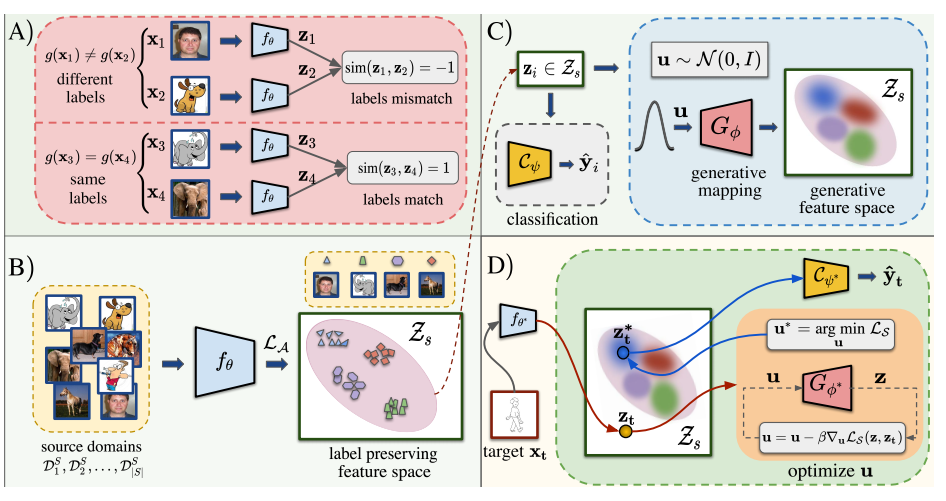
\includegraphics[width=0.7\textwidth]{fig1.png}
    \caption{A) We design a function f (neural network fθ) to learn a label-preserving metric that produces a similarity score
of 1 when the ground truth labels (given by function g) between a pair of images match and -1 otherwise. The function
‘sim’ refers to the cosine similarity function. B) f is implemented using a neural network fθ. During training, the examples
from the source domains are utilized to create a source manifold Zs using loss LA such that the features on the manifold
are implicitly clustered to preserve the labels of examples. C) A classifier Cψ and a generative model Gφ are trained on the
label-preserving features from manifold Zs such that Gφ learns to map a Gaussian vector u to a point on the manifold Zs.
D) During inference, fθ∗ projects target xt to a point zt on the label-preserving feature space. We propose an inference-time
procedure to project the target feature to a point z∗ t on the source manifold which is finally classified to predict its label ˆyt. indicate that the weights of their corresponding networks are fixed during inference.}
    \label{fig:fig1}
\end{figure*}

\section{Proposed Method}
\subsection{Problem Setting and Method Overview}
Let  $\chi$ and Y respectively denote data and the label
spaces. Let H be the space of hypotheses where each hypothesis h in H maps points from X to a label in Y. A
domain is defined by the tuple (D, gD) where D is a probability distribution over X and gD where $gD : X → Y $is
a function that assigns ground-truth labels. It is generally
assumed that the ground-truth labeling function g is same
across all the domains. Domain Generalization is defined as
the task where there are a total of N domains out of which
|S| are source and |T| are target domains. The source and
target domains are respectively denoted by DiS, $i ∈ [|S|]$
and $DTj , j ∈ [|T|].$ The objective is to train a classifier on
the source domains that predicts well on the target domain
when the target samples are not available during training. \par
The motivation for our method comes from the following observation: DG methods that learn domain invariant
representations do so only using the source data. Therefore,
classifiers trained on such representations are not guaranteed to perform well on target data that is outside the source
data manifolds. Hence, performance on the target data can
be improved if the target sample is projected on to the manifold of the source features such that the ground-truth label
is preserved, before classification. To this end, we propose
a three-part procedure for domain generalization: \\

\begin{enumerate}
    \item \textbf{(Training):} Learn a label-preserving domain invariant
representation using source data. We first transform the data
from multiple source domains into a space where they are
clustered according to class labels, irrespective of the domains and build a classifier on these features.
 \item \textbf{(Training):} Learn to generate features from the domain
invariant feature manifold created from the source data by
constructing a generative model on it.
 \item \textbf{(Inference):} Given a test target sample, project it on
to the source-feature manifold in a label-preserving manner. This is done by solving an inference-time optimization
problem on the input space of the aforementioned generative model. Finally, classify the projected target feature.
\end{enumerate}

Note that the parameters of all the networks involved
(Feature extractor, generative model and the classifier) are
learned only using the source data and fixed during inference. Thus, our approach is well within the realm of DG despite a label-preserving optimization problem being solved
for every target sample during inference. The overall procedure is depicted in Figure 1. In the subsequent sections,
we describe all the aforementioned components in detail.

%-------------------------------------------------------------------------
\subsection{Label-Preserving Transformation}
\subsubsection{Domain invariant Features}
The first step in our method is to learn a feature (metric)
space such that the input images are clustered in accordance
with their labels (classes) irrespective of their domains. We
explicitly construct such a feature space F with a function
$ f: \chi \longrightarrow F $ by solving the following optimization problem.
\begin{equation}
 \sum_{j=1}^{N} \sum_{i=1}^{N}   (-1)^{\alpha(i,j)} \|f(x_i) - f(x_j)\|^2
\end{equation}



The function f is learned such that when a pair of source
samples have the same ground truth labels, the norm of the
difference between their representations under f is low irrespective of their domain membership and high when they
belong to different classes. Under this formulation, the features in the space F will be ‘clustered’ in accordance with
their class labels, irrespective of the domains. In fact, it
can be shown that the aforementioned f minimizes the Hdivergence [2] between any two pairs of domains.

\textbf{Proposition 1.} \textit{The label-preserving transformation f defined in Eq. 1, reduces the H-divergence between any two
pair of domains on which it is learned (Proof in Appendix).}

In summary, the proposed feature transformation merges
multiple source domains into a single feature domain such
that images that have the same labels cluster into a group in
the feature space.

\subsubsection{Learning the f-function}
We propose to learn f by parameterizing it with a deep neural network, fθ. It is easy to see that the objective function in Eq. 1 reduces to an optimization of cosine-similarity
between the pair of samples $fθ(xi)$ and $fθ(xj)$ Suppose
$zi = fθ(xi)$ and $zj = fθ(xj)$ represent the feature vectors of inputs, the cosine-similarity si,j between zi and zj
is given by,
\begin{equation}
    S_{i,j} = \frac{z_i . z_j}{\|z_i\|  \|z_j\| }
\end{equation}

Note that the optimization problem in Eq. 1 seeks si,j to
be high when the labels are same and low when they are
different (denoted by the α(i, j) term in Eq. 1). Thus,
we first translate si,j into logits for a sigmoid activation
and use binary cross entropy on the generated probabilities. However, since −1 ≤ si,j ≤ 1, we scale it with
a small positive constant τ (typically 0.1) to widen the
range of the generated logits. Mathematically, we can write
$pi,j = sigmoid(si,j/τ).$ Under this formulation, one can
treat pi,j as a similarity score which should be 1 if (xi, xj)
have the same label (α(i, j) = 0) and 0 otherwise. Thus,
we finally use a binary cross entropy loss LA between pi,j
and 1 − α(i, j), to train the fθ network.

\subsection{Inference-time Target Projections}

In a DG setting, the feature transformation mentioned
in the previous sections is learned on the source domains.
Let Zs denote the manifold created by learning such features using the source data. The classifier Cψ is trained on
points from the source data feature manifold Zs. Because
of the domain shift, the feature f(xt) corresponding to a
test target point xt might not fall on the source data feature manifold Zs. This causes the classifier to fail on the
target feature $f(xt)$. To address this issue, we propose to
project or ‘push’ the target feature onto Zs while preserving
the ground truth label of xt, so that the classifier can better
discern the class label of xt. We propose to accomplish
such a label-preserving projection by solving an inferencetime optimization problem on the input space of a generative model trained on Zs. For convenience, we define a
function


\subsubsection{Generating the Source-Feature Manifold Zs}
Once the label-preserving source-feature manifold Zs is obtained through fθ, we build a generative model on it. That
is, a transformation from samples from an arbitrary distribution, such as Normal distribution, to the source-data feature
manifold Zs is learned. We choose two state-of-the-art neural generative models for this purpose: (a) Variational AutoEncoder (VAE) [18]: In this setting, a VAE is trained using the source-data features z, by encoding them to produce
the latent space u ∼ N (0, I). A decoder Gφ reconstructs
(generates) the source-feature manifold Zs by minimizing
a regularized norm-based loss. (b) Generative Adversarial Networks (GAN) [11]: Here, a GAN is trained with a
generator network Gφ that maps an arbitrary latent space u ∼ N (0, I) to the source-feature manifold Zs. Note that
these generative models are trained on the source-features
alone and fixed during the inference procedure. We denote
the trained generative model by Gφ∗.
\subsubsection{Label-preserving Projections}
The final component of our method is to project the target features on to the source-feature manifold during inference. It is to be noted that the transformation fθ is constructed such that when a pair of samples have zero distance
in that space, they have same ground truth label. That is, if
kfθ(x1) − fθ(x2)k = 0, then g(x1) = g(x2). We exploit
this property and solve a (per-sample) optimization procedure on the input space of the generative model Gφ∗(u) to
obtain the target-feature projection. \par
Let zt = fθ(xt) denote the feature vector corresponding to a test target sample xt. Our goal is to find the projected target feature in the source-feature manifold z∗ t ∈ Zs
that has the same ground-truth label as that of zt. By construction of fθ (Eq. 1), the cosine distance between zt and
z∗
t should be low if their ground truth labels are to match.
Based on this, we devise the following optimization problem on the input space of Gφ∗ to find z∗ t:


The objective function in Eq. 4 seeks to find the projected
target feature z∗ t (via u∗ from Eq. 5) whose cosine distance is least from the true target feature zt. The implicit
assumption of our method is that when the target example
is projected on to the source manifold, minimizing distance
is equivalent to preserving labels.

\subsubsection{Analysis and Implementation}
In this section, we analyze the performance of the classifier
on account of it using the projected target instead of the real
target features. We start by upper bounding the expected
value of the misclassification when the projected target is
used in the classifier, in the below preposition.

\textbf{Proposition 2.} \textit{The expected misclassification rate obtained with a classifier h when the projected target is used
instead of the true target, obeys the following upper-bound: 
where D and DT ∗ respectively denote the true and the projected target distributions respectively (Proof in Appendix).}

The term (i) in Eq. 6 is the misclassification error of h
on the projected target and term (ii) is the difference between the ground truth labels of the true and the projected
targets. Given that our overall objective is to minimize the
LHS of Eq. 6, the optimization procedure in the previous
section aims to minimize term (ii) while term (i) is expected
to be less since the projected target is expected to lie on
the source-feature manifold Zs on which the classifier is
trained. \par
In the implementation, during inference, we optimize the
objective in Eq. 4 (reducing term (ii) in Eq. 6) by gradient
descent. A discussion on the choice of stopping criteria can
be found in Section 4.7. The training and the inference procedures are detailed in Algorithm 1 and shown in Figure 1.


\section{Experiments and Results}
We have considered four standard DG datasets - PACS
[21], VLCS [8], Office-Home [43] and Digits-DG [48] to
demonstrate the efficacy of our method. All these datasets
contain four domains out of which three are used as sources
and the other as a target in a leave-one-out strategy. We use
a VAE as the generative model Gφ in all our main results
owing to its stability of training vis-a-vis a GAN. The performance metric is the classification accuracy and we compare against a baseline Deep All method: classifier trained
on the combined source domains without employing any
DG techniques. For each target domain, we have reported
our average and standard deviation for five independent runs
of the model. We also compare our method with the existing DG methods and report the results, dataset wise. We
report the standard deviation as 0 for models which have
not reported them. For each dataset, we use the validation
set for selecting hyperparameters if it is available. Otherwise, we split the data from source domains and use thesmaller set for hyperparameter selection. We also use dataaugmentation for regularizing the network fθ. For further
details on the datasets, machine configuration and choice of
hyperparameters, please refer to the Appendix.

\begin{table}
\small
  \label{tab:tab1}
  \begin{tabular}{lccccl}
   \hline
    Method & Art &Cartoon & Sketch & Photo &Avg\\
    \hline
    \multicolumn{6}{c}{AlexNet} \\
    \hline
   Deep All & \small{65.69+0.2} &65.69+0.2 &65.69&65.69+0.2 & 71.20 \\ \hline
   Deep All & 65.69+0.2 &65.69+0.2 &65.69+0.2&65.69 & 71.20 \\ \hline
   Deep All & 65.69+0.2 &65.69+0.2 &65.69+0.2&65.69 & 71.20 \\ \hline
   Deep All & 65.69+0.2 &65.69+0.2 &65.69+0.2&65.69 & 71.20 \\ \hline
   Deep All & 65.69+0.2 &65.69+0.2 &65.69+0.2&65.69 & 71.20 \\ \hline
   Deep All & 65.69+0.2 &65.69+0.2 &65.69+0.2&65.69 & 71.20 \\ \hline
   \multicolumn{6}{c}{Resnet-18} \\
    \hline
     Deep All & \small{65.69+0.2} &65.69+0.2 &65.69&65.69+0.2 & 71.20 \\ \hline
   Deep All & 65.69+0.2 &65.69+0.2 &65.69+0.2&65.69 & 71.20 \\ \hline
   Deep All & 65.69+0.2 &65.69+0.2 &65.69+0.2&65.69 & 71.20 \\ \hline
   Deep All & 65.69+0.2 &65.69+0.2 &65.69+0.2&65.69 & 71.20 \\ \hline
   Deep All & 65.69+0.2 &65.69+0.2 &65.69+0.2&65.69 & 71.20 \\ \hline
   Deep All & 65.69+0.2 &65.69+0.2 &65.69+0.2&65.69 & 71.20 \\ \hline
   \multicolumn{6}{c}{ResNet-50} \\
    \hline
     Deep All & \small{65.69+0.2} &65.69+0.2 &65.69&65.69+0.2 & 71.20 \\ \hline
   Deep All & 65.69+0.2 &65.69+0.2 &65.69+0.2&65.69 & 71.20 \\ \hline
   Deep All & 65.69+0.2 &65.69+0.2 &65.69+0.2&65.69 & 71.20 \\ \hline
   Deep All & 65.69+0.2 &65.69+0.2 &65.69+0.2&65.69 & 71.20 \\ \hline
   Deep All & 65.69+0.2 &65.69+0.2 &65.69+0.2&65.69 & 71.20 \\ \hline
   Deep All & 65.69+0.2 &65.69+0.2 &65.69+0.2&65.69 & 71.20 \\ \hline
\end{tabular}
\caption{Comparison of performance between different
models on PACS [21] dataset with AlexNet, ResNet-18 and
ResNet-50 as backbones for the fθ network.}
\end{table}

\subsection{Multi-source Domain Generalization}
\textbf{Digits-DG:} The PACS dataset consists of images from Photo,
Art Painting, Cartoon and Sketch domains. We follow the
experimental protocol defined in [21]. We use ResNet-50,
ResNet-18 and AlexNet as backbones for the feature extractor network fθ and train them on source domains. To perform target projection, we learn to sample from the features
produced by fθ by training a VAE on the latent space (u).
We achieve state-of-the-art results with all three choices of
backbones as shown in Table 1.
\textbf{Digits-DG:} VLCS comprises of the VOC2007(Pascal),
LabelMe, Caltech and Sun domains, all of which contain
photos. We follow the same experimental setup as mentioned in [27] where we train on three source domains with
70% data from each and test on all the examples from the
fourth target domain. We utilize similar setup for fθ and Gφ
as in the PACS dataset with AlexNet as the backbone. We
achieve SOTA results on VLCS as evident from Table 2. We
emphasize that unlike PACS dataset where the domains differ in image styles, VLCS consists of domains that contain
only photos. Thus, we demonstrate that our method generalizes well even when the source domains are not diverse.

\begin{table}[t]
\small
  \label{tab:tab2}
  \begin{tabular}{lccccl}
   \hline
    Method & Caltech &Labelme & Pascal & Sum &Avg\\
    \hline
   Deep All & \small{65.69+0.2} &65.69+0.2 &65.69&65.69+0.2 & 71.20 \\ \hline
   jigen & 65.69+0.2 &65.69+0.2 &65.69+0.2&65.69 & 71.20 \\ \hline
   MMLD & 65.69+0.2 &65.69+0.2 &65.69+0.2&65.69 & 71.20 \\ \hline
   Deep All & 65.69+0.2 &65.69+0.2 &65.69+0.2&65.69 & 71.20 \\ \hline
   Deep All & 65.69+0.2 &65.69+0.2 &65.69+0.2&65.69 & 71.20 \\ \hline
   Deep All & 65.69+0.2 &65.69+0.2 &65.69+0.2&65.69 & 71.20 \\ \hline
\end{tabular}
\caption{Comparison of performance between different
models using AlexNet backbone on VLCS [8] dataset.}
\end{table}
\begin{table}
\small
  \label{tab:tab3}
  \begin{tabular}{lccccl}
   \hline
    Method & Artistic & Clipart & Product & Real World &Avg\\
    \hline
   Deep All & \small{65.69+0.2} &65.69+0.2 &65.69&65.69+0.2 & 71.20 \\ \hline
   jigen & 65.69+0.2 &65.69+0.2 &65.69+0.2&65.69 & 71.20 \\ \hline
   MMLD & 65.69+0.2 &65.69+0.2 &65.69+0.2&65.69 & 71.20 \\ \hline
   Deep All & 65.69+0.2 &65.69+0.2 &65.69+0.2&65.69 & 71.20 \\ \hline
   Deep All & 65.69+0.2 &65.69+0.2 &65.69+0.2&65.69 & 71.20 \\ \hline
   Deep All & 65.69+0.2 &65.69+0.2 &65.69+0.2&65.69 & 71.20 \\ \hline
    Deep All & 65.69+0.2 &65.69+0.2 &65.69+0.2&65.69 & 71.20 \\ \hline
     Deep All & \textbf{65.69+0.2} &\textbf{65.69+0.2} &\textbf{65.69+0.2}&\textbf{65.69+0.2} & \textbf{65.69+0.2} \\ \hline
\end{tabular}
\caption{Comparison of performance between different
models using ResNet-18 backbone on Office-Home [43].}
\end{table}


\textbf{Digits-DG:} Office-Home contains images from 4 domains namely Artistic, Clipart, Product and Real-World.
We follow the experimental protocol as outlined in [7]. We
utilize a ResNet-18 as backbone with two additional fullyconnected layers. The reconstruction error in VAE is minimized using both L1 and L2 loss functions. We achieve
SOTA results on all the domains using a ResNet-18 backbone as shown in Table 3. It should be noted that Clipart is
a difficult domain to generalize to as it is dissimilar to other
domains. We achieve 5.6% improvement over the nearest
competitor on the Clipart domain, showcasing the merit of
our method in generalizing to dissimilar target domains.

\textbf{Digits-DG:} Digits-DG is the task of digit recognition using MNIST [20], MNIST-M [9], SVHN [32] and SYN [9]
domains that differ drastically in font style and background.
We follow the experimental setup of [48] and use their architecture for the feature extractor fθ. The Gφ network
is implemented in a similar way as it is implemented for
the PACS dataset with ResNet-18 as the backbone. Table 4
shows the performance of our method on Digits-DG dataset
compared against various SOTA methods.

\subsection{Pairwise H-divergence}
We examine the effectiveness of the proposed method
in projecting target features onto the source-feature manifold by computing a proxy measure for H-divergence called
the A-distance [3], that measures the divergence between
two domains. We compute the A-distance between features
from the Sketch domain (target domain) and each of the
three source domains (Photo, Cartoon and Art), obtained in
two ways - first, from a ResNet-18 model trained on the
source domains (Deep All), and second, the features obtained after performing target projections using our method.
We compare the A-distance obtained from these two methods in Figure 2a . It is observed that the source-target divergence is reduced substantially compared to Deep All, suggesting the effectiveness of our projection scheme in bringing the target points onto the source manifold.

\subsection{Ablation Studies}
To quantify the importance of the two components (i.e.
the networks fθ and Gφ), we perform ablative studies using
the Office-Home and Digits-DG datasets. For the OfficeHome dataset, the Deep All model is trained with ResNet-
18 as the backbone while the backbone proposed by [48] is
used for the Deep All model on the Digits-DG dataset. We
classify target domain features extracted from the feature
extractor network without the target projection procedure
as shown in Figure 2b. We observe a marginal improvement over Deep All by classifying on the domain-invariant
features learnt by fθ without using the Gφ network. We
attribute this to the explicit class separability imposed by
the fθ network in the feature space F. When we exclude
the fθ network by training the generative model on Deep
All features and perform the projection procedure on these
features, we still observe a sizable performance boost over
merely classifying with the Deep All model. This shows the
effectiveness of the target projection procedure as a sampling strategy. The best performance is achieved with all
components working together as seen in Figure 2b.

\subsection{Sampling strategy}
To quantify the effect of the specific generative model
used for the Gφ network, we report performance with three
samplers on VLCS dataset, namely: (a) VAE, (b) 1-Nearest
Neighbor (1-NN) of the target sample with the source samples using the similarity metric as in Eq. 2, (c) GAN, and
show results in Table 5. It is seen that sampling using continuous generative models (VAE and GAN) offer better performance compared to 1-NN sampling. On domains like
LabelMe and Sun, they offer improvement of about 5.7%
and 7.0% respectively over the 1-NN method of sampling.
This is attributed to the fact that generative models can approximate the true data distribution by learning from empirical data and offer infinite sampling while 1-NN search
is restricted to the existing training points only.


\begin{figure*}[t]
    \centering
    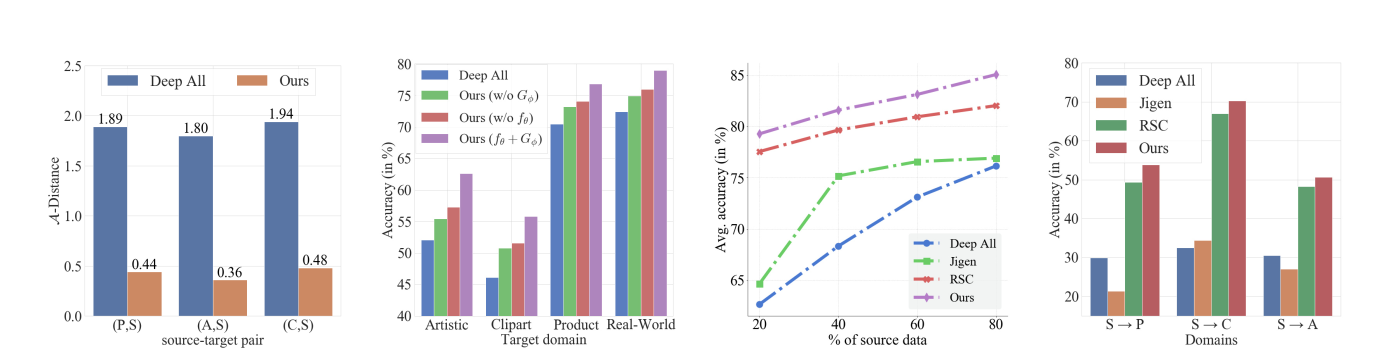
\includegraphics[width=\textwidth]{fig2.png}
    \caption{ (left to right) (a) Plot showing A-divergence between source and projected target features. (b) Ablation on OfficeHome dataset highlighting the relative importance of different components employed in our method. (c) Relative performance
of different methods trained on 20%, 40%, 60% and 80% of PACS dataset. For each setting, we report average performance
with all examples from the target domains using leave-one-out strategy. (d) Relative performance of DG methods trained on
a single domain (Sketch (S)) and tested on Photo (P), Cartoon (C) and Art (A) domains.}
    \label{fig:fig2}
\end{figure*}
\subsection{Low resource settings}
In this section, we demonstrate the efficacy of our
method in low-resource settings. We show that our method
generalizes well when used in scarce resource settings and
single domain DG problems, and can also easily be extended to supervised domain adaptation with access to scant
labelled target samples. Our method has a two-fold advantage that makes it especially data-efficient: (a) since fθ is
trained on pairs of images, it can learn effectively even on
small datasets (b) the generative model Gφ enables infinite
sampling during the target projection procedure.
\subsubsection{Scarce resource setting}
We compare our method against Deep All and two state-ofthe-art methods, RSC [16] and Jigen [5]. For each source
domain in PACS we train on data
from each domain and test on the entire target domain.
From Figure 2c, it is evident that our method outperforms
all the baselines at every considered resource setting.
\subsubsection{Supervised Domain Adaptation}
This setting has also been referred to as Few-shot Domain
Adaptation in [36] and [28]. In this setting, in addition to
the source data, we assume that we have access to a limited
number of labelled samples (|T |) from the target domain at
train time. We train the feature extractor network fθ, generative model Gφ and the classifier Cψ on the source data and
fine tune on the target samples. We compare our method
against M-ADA [36] and FADA [28] on the Digits dataset.
The results are presented in Table 6. We outperform our
nearest competitors by a significant margin, thus highlighting the adaptability of our method to this use-case.
\subsubsection{Single Source Domain Generalization}
In single source DG, we only have access to a single domain
during training and aim to generalize to all other unseen domains. We train on the Sketch domain of the PACS dataset
and test on the other three domains (i.e. Photo, Art Painting
and Cartoon). We compare our method against Jigen [5] and
RSC [16]. The results are presented in Figure 2d. We also
examine the individual effects of each of the components fθ
and Gφ of our method in this scenario by examining the performance without each of them (Table 7). We observe that
without Gφ, the performance difference between Deep All
and our method is substantially lower than the improvement
obtained by performing target projections on Deep All features, highlighting the effectiveness of the projection procedure. The best performance is obtained when both are used
together, since the projection procedure effectively utilizes
the label-preserving metric defined by fθ.

\begin{figure}[t]
    \centering
    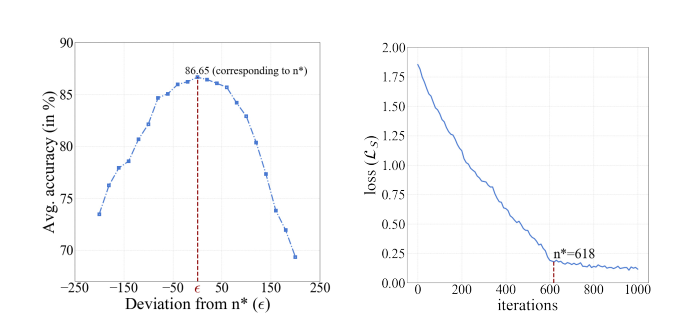
\includegraphics[width=0.5\textwidth]{fig3.png}
    \caption{ (left) (a) Effect of deviation from the optimal
number of iterations of each target example during inference on PACS. (right) (b) Plot of iterations vs loss for projection of a target example from Sketch domain on source
manifold (Zs) created by Photo, Art and Cartoon domains.}
    \label{fig:fig3}
\end{figure}

\begin{figure}[t]
    \centering
    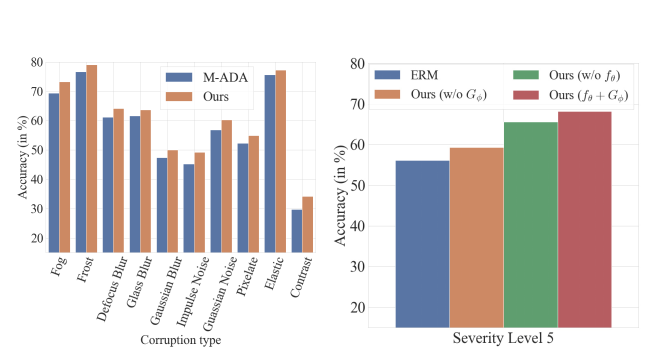
\includegraphics[width=0.5\textwidth]{fig4.png}
    \caption{ (left) (a) Performance comparison between MADA and our method on 10 out of the 19 corruption types
at severity level 5 from the CIFAR-10-C dataset. (right)
(b) Plot showing relative importance of each component of
our method on the CIFAR-10-C dataset. Accuracy averaged
over all 19 corruption levels.}
    \label{fig:fig4}
\end{figure}





\subsection{Robust Domain Generalization}
We examine the robustness of our method against different types of corruptions. We benchmark against the CIFAR-
10-C dataset [12], which consists of images with 19 corruptions types applied at five levels of severities on the test
set of CIFAR-10. We follow the protocol detailed in [36]
and train our model on the CIFAR-10 dataset using a Wide
Residual Network (WRN) backbone [46]. The results are
presented severity level-wise in Table 8 and by type of corruption in Figure 4a. Similar to 4.5.3, we observe the effectiveness of Gφ in generalizing to corruptions.
\subsection{Robust Domain Generalization}

We address this issue heuristically: stop the iteration process at the “elbow-point” (maxima of the second derivative)
of the loss curve as a function of the number of iterations
(denoted by n∗). This choice is inspired by the observation that the elbow-point reflects the point of diminishing
returns; for a constant iteration rate (β), the loss decreases
at a slower rate beyond this point.\par
As empirical evidence, we vary the stopping point for
each target sample by a fixed number of iterations ǫ around
the maxima n∗ of the second derivative values of the sample
and calculate the accuracy on the target projections so obtained. The plot of accuracy vs ǫ is shown in Figure 3a. We
observe that the highest accuracy is obtained around ǫ = 0
which indicates the correctness of the stopping criteria n∗.
For negative values of ǫ, the accuracy drop can be explained
by inadequate label preservation, while the projected target
leaves the source manifold for positive values of ǫ.
\section{Conclusion}
We propose a novel Domain Generalization technique
where the source domains are utilized to learn a domain
invariant label-preserving metric space. During inference,
every target sample is projected onto this space so that the
classifier trained on the source features can generalize well
on the projected target sample. We have demonstrated that
this method yields SOTA results on Multi Source, Single
Source and Robust Domain Generalization settings. In addition, the data-efficiency of the method makes it suitable
to work well in Low Resource settings. Future iterations of
work could attempt to extend this method to Domain Generalization for Segmentation and Zero-Shot Learning.

\section{References}

{\small
\bibliographystyle{ieee_fullname}
\bibliography{egbib}
}

\end{document}
